\chapter{Theoretical Background} 	% Produces section heading.  Lower-level
\label{theoretical-background}

%Basics such as theory, definitions, relevant theories, related work and state of the art should be included here.

In this chapter,
the theoretical background which is needed for comprehending the topic, problem,
and discussed material
within this thesis,
is presented.
It consists of general definitions of terms and concepts,
as well as various background information.

% maximal 1.1.1 
% wenns 1.1 gibt, muss es auch 1.2 geben

\section{General Definitions}
\label{theoretical-background:general-definitions}

The following section includes general definitions of terms on the topic.

\subsection{GitOps}

Infrastructure-as-Code which is stored in a Git repository,
and executed by a workflow system,
is not actually the concept behind GitOps.
A visual representation of what is not GitOps can be seen in
fig. \ref{fig:iac-is-not-gitops}.
Infrastructure-as-Code is only one aspect of GitOps, namely the declarative one.
There are three more principles of GitOps.
%The definition of GitOps
%is stated in section \ref{theoretical-background:general-definitions} of this thesis.

\begin{figure}[h]
	\centering
	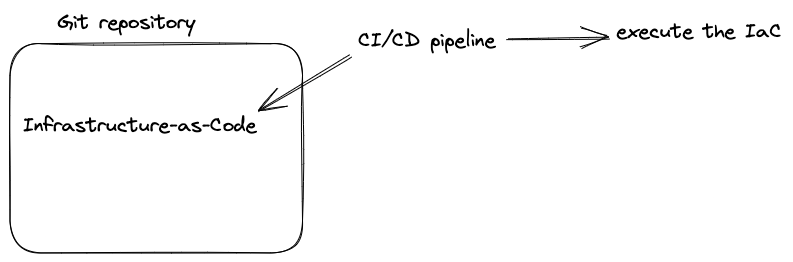
\includegraphics[width=1.00\linewidth]{assets/iac-is-not-gitops.png}
	\caption{Infrastructure-as-Code is not GitOps.
		%		(\citeauthor{ref}, \citeyear{ref}).
	}
	\label{fig:iac-is-not-gitops}	
\end{figure}

% TODO: in indirektes Zitat umwandeln
%Moreover, unlike DevOps,
%\begin{quotation}
%	\noindent
%	\enquote*{GitOps is not intended to tackle the fuzzier area of social interactions and culture. [...] GitOps is ultimately meant to be a technology pattern, not a social practice. [...] Fundamentally, all the social aspects should be derived from the technical principles. Git is designed as a team tool and gives you a social context, because you have metadata, committed workflows, and group activities. But GitOps is not supposed to be a social movement. [...] With GitOps, all changes to infrastructure and application deployment are versioned, immutable, auditable, and reversible. [...] GitOps is about automating operations and shifting left, so that developers can perform operations tasks without having to always understand it in detail. [...] With GitOps, developers use tools like git to cause operational changes in a robust manner, allowing platform teams to focus on core platform engineering and operations, and leaving developers to focus on product, customers, rapid development, user satisfaction, and so on.}
%	\autocite{definingGitOpsGithubReadmeFeatured}
%\end{quotation}

%To conclude, Infrastructure-as-Code is not GitOps. IaC is just one aspect of GitOps.

To avoid confusion with what GitOps actually is, 
the OpenGitOps project
\autocite{openGitOpsProject}
was created within the CNCF;
which is maintained by the GitOps working group.
The overall goal of OpenGitOps is to establish a clear vendor-neutral,
principle-driven meaning of GitOps,
which shall provide a foundation for interoperability between tools, conformance and certification through enduring programs, documents and code
\autocite{opengitopsDocuments}.
In fig. \ref{fig:gitOpsConcept} a visual representation can be seen of the main GitOps concept.

\begin{figure}[h]
	\centering
	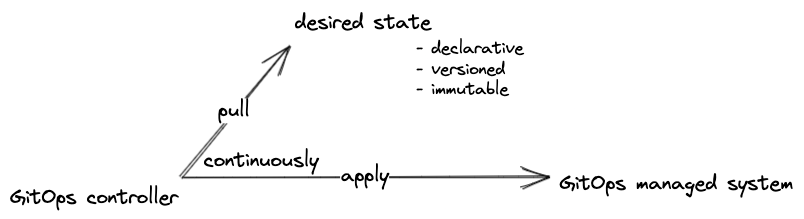
\includegraphics[width=1.00\linewidth]{assets/gitops-concept.png}
	\caption{GitOps concept.
		%		(\citeauthor{ref}, \citeyear{ref}).
	}
	\label{fig:gitOpsConcept}	
\end{figure}

%This thesis aims at adhering to the definition of the term GitOps,
%as specified by the CNCF project OpenGitOps.
%The overall goal of OpenGitOps is to establish a clear vendor-neutral,
%principle-driven meaning of GitOps,
%which shall provide a foundation for interoperability between tools, conformance and certification through enduring programs, documents and code
%\autocite{opengitopsDocuments}.

\noindent
\enquote*{The primary four principles
	for the desired state of a
	system managed by GitOps are the following} \autocite{gitopsPrinciplesv100}:

\begin{itemize}
	\item \textbf{Declarative} \\
	\enquote*{A system managed by GitOps must have its desired state expressed declaratively.}
	\item \textbf{Versioned and Immutable} \\
	\enquote*{Desired state is stored in a way that enforces immutability, versioning and retains a complete version history.}
	\item \textbf{Pulled Automatically} \\
	\enquote*{Software agents automatically pull the desired state declarations from the source.}
	\item \textbf{Continuously Reconciled} \\
	\enquote*{Software agents continuously observe actual system state and attempt to apply the desired state.}
	\autocite{gitopsPrinciplesv100}
\end{itemize}

% ensure list does not span over multiple pages in PDF export

These principles are defined in OpenGitOps version 1.0.0,
along with glossary
\autocite{gitopsGlossary}
for associated terms and concepts.
%The ones needed for understanding of this thesis,
%are the following:

\enquote*{\textbf{Continuous} is intended to match the industry standard term: reconciliation continues to happen, not that it must be instantaneous.} \autocite{gitopsGlossary}

\textbf{Declarative Description}:
\enquote*{A configuration that describes the desired operating state of a system without specifying procedures for how that state will be achieved. This separates configuration (the desired state) from the implementation (commands, API calls, scripts etc.) used to achieve that state.}
\autocite{gitopsGlossary}


\textbf{Desired State}:
\enquote*{The aggregate of all configuration data that is sufficient to recreate the system so that instances of the system are behaviourally indistinguishable. This configuration data generally does not include persistent application data, eg. database contents, though often does include credentials for accessing that data, or configuration for data recovery tools running on that system.}
\autocite{gitopsGlossary}

\textbf{Drift}:
\enquote*{When a system's actual state has moved or is in the process of moving away from the desired state, this is often referred to as drift.}
\autocite{gitopsGlossary}

\textbf{Feedback}:
\enquote*{Open GitOps follows control-theory and operates in a closed-loop. In control theory, feedback represents how previous attempts to apply a desired state have affected the actual state. For example if the desired state requires more resources than exist in a system, the software agent may make attempts to add resources, to automatically rollback to a previous version, or to send alerts to human operators.}
\autocite{gitopsGlossary}

\textbf{Reconciliation}:
\enquote*{The process of ensuring the actual state of a system matches its desired state. Contrary to traditional CI/CD where automation is generally driven by pre-set triggers, in GitOps reconciliation is triggered whenever there is a divergence. Divergence could be due to the actual state unintentionally drifting from the desired state declarations, or a new desired state declaration version having been changed intentionally. Actions are taken based on policies around feedback from the system and previous reconciliation attempts, in order to reduce deviation over time.}
\autocite{gitopsGlossary}

\textbf{Software System}:
\enquote*{A software system managed by GitOps includes} \autocite{gitopsGlossary}:
\begin{itemize}
	\item \enquote*{One or more runtime environments consisting of resources under management}
	\item \enquote*{The management agents within each runtime}
	\item \enquote*{Policies for controlling access and management of repositories, deployments, runtimes}
	\autocite{gitopsGlossary}
\end{itemize}

\textbf{State Store}:
\enquote*{A system for storing immutable versions of desired state declarations. This state store should provide access control and auditing on the changes to the Desired State. Git, from which GitOps derives its name, is the canonical example used as this state store but any other system that meets these criteria may be used. In all cases, these state stores must be properly configured and precautions must be taken to comply with requirements set out in the GitOps Principles.}
\autocite{gitopsGlossary}







\subsection{Release}

A release in the context of this thesis
represents the process of
publishing a new version of an application or software component
to the users.
When following GitOps practices,
this usually means
pushing a new Git tag to a Git repository,
which triggers a CI/CD workflow,
which as one of its steps publishes the software artifact of
the new version of the application in an artifact registry.

\subsection{Promotion}

Promotion in the context of this thesis is defined as
the process of promoting a new application or infrastructure version (release)
to another deployment environment.
In the context of GitOps and Git repositories,
this often means changing declarative definitions of the desired state in Git repositories.

\subsection{Environment}

An Environment
- or GitOps Environment -
in the context of this thesis
is defined as a target deployment environment for a given application;
e.g. Development, Testing, or Production.
Most of the time this is a Kubernetes cluster or namespace.

In the context of the proposed Kubernetes Custom Resource Definition
Environment, however it represents a folder/directory in a Git repository,
which points to a deployment environment or cluster/namespace as defined
in the previous paragraph.







%\subsection{Other Terms}
%
%\subsubsection*{Cloud Native Application}
%
%\begin{quotation}
%	\noindent
%	\enquote*{A cloud-native application (CNA) is a distributed, elastic and horizontal scalable system composed of (micro)services which isolates state in a
%		minimum of stateful components. The application and each self-contained
%		deployment unit of that application is designed according to cloud-focused
%		design patterns and operated on a self-service elastic platform.}
%	\autocite{cloudNativeApplicationDefinition2017}
%\end{quotation}





%\subsection*{Internal Developer Platform}
%
%\begin{quotation}
%	\noindent
%	\enquote*{An Internal Developer Platform (IDP) is built by a platform team to build golden paths and enable developer self-service. An IDP consists of many different techs and tools, glued together in a way that lowers cognitive load on developers without abstracting away context and underlying technologies. Following best practices, platform teams treat their platform as a product and build it based on user research, maintain and continuously improve it.}
%	\autocite{internaldeveloperplatformWhatIsIDP}
%\end{quotation}

%\subsection*{Platform Engineering}
%
%Platform Engineering represents the engineering processes
%for providing an internal developer platform (as defined in this section).








%\subsection*{Cloud Computing}
%
%\begin{quotation}
%\noindent
%\enquote*{Cloud computing is a model for enabling ubiquitous, convenient, on-demand network access to a shared
	%	pool of configurable computing resources (e.g., networks, servers, storage, applications, and services) that
	%	can be rapidly provisioned and released with minimal management effort or service provider interaction.
	%	This cloud model is composed of five essential characteristics, three service models, and four deployment
	%	models.}
%\autocite{cloudComputingNistDefinition2011}
%\end{quotation}
%
%The characteristics are
%\autocite{cloudComputingNistDefinition2011}:
%
%\begin{itemize}
%	\item On-demand self-service
%	\item Broad network access
%	\item Resource pooling
%	\item Rapid elasticity
%	\item Measured service
%\end{itemize}
%
%The service models are
%\autocite{cloudComputingNistDefinition2011}:
%
%\begin{itemize}
%	\item Software as a Service (SaaS)
%	\item Platform as a Service (PaaS)
%	\item Infrastructure as a Service (IaaS)
%\end{itemize}
%
%The deployment models are
%\autocite{cloudComputingNistDefinition2011}:
%
%\begin{itemize}
%	\item Private cloud
%	\item Community cloud
%	\item Public cloud
%	\item Hybrid cloud
%\end{itemize}









\section{DevOps}

\citeauthor{devopsDefinition2016} (\citeyear{devopsDefinition2016})
define DevOps as
a development methodology aimed at bridging the gap between
development and operations, emphasizing communication and collaboration,
continuous integration, quality assurance and delivery with automated deployment
utilizing a set of development practices
\autocite{devopsDefinition2016}.

%DevOps is seeing increasingly more adoption amongst organizations.
One of the most important principles of DevOps is
to allow the developer who brings new code changes
which end up in new product releases,
to have as much insight into the software development lifecycle as possible.
So it is not just bringing developers and operations closer together,
but to shift many processes into the developers hands.
This is to give developers as much insight as possible,
in order to decrease efficiency and productivity to eventually
decrease the time-to-market for new product releases, features and bug fixes.
This is essentially needed for organizations to continue to thrive in todays
rapidly changing world.

Cloud native technologies have allowed for this movement to happen.
An important aspect of cloud technologies is the self-service.
When previously it was necessary to have many different teams and departments
within a software development organization,
each being responsible for individual parts of the 
software development lifecycle,
it is now easier than ever before possible to reduce the amount of
teams down to a minimum, in order to reduce friction between people communications and processes.
This additionally gives the developers much better insights of what effect their code changes have
on the end product or service, which users consume.

%In order to increase the level of self-service for developers,
%and increase their productivity,
%many organizations implement the concept of internal developer platforms.
%While this concept has been around for quite a while,
%it has now in recent years explicitely gotten more meaning and attention.
%
%Internal Developer Platforms have received a lot of attention
%when Spotify released their project Backstage
%\autocite{backstageIOWebsite}
%with an open-source license in 2020. The project was accepted into the CNCF in 2022.
%
%%
%Backstage was initially created at Spotify, due to the need for it.
%As Spotify grew and added increasingly more microservices to their software catalog,
%their developers were observed to becoming less and less productive.
%Engineering teams at Spotify were spending too much time context switching between
%a burden of tasks, which were the result of bad organization of all their
%information around applications, microservices, infrastructure, etc.
%What was actually valuable, building, testing and releasing code,
%was becoming less frequent and more difficult to achieve over time.
%Engineers at Spotify decided that they needed to make it easier 
%for their developers to do their work
%\autocite{backstageSpotifyStory}.
%
%Their idea was to
%\enquote*{centralize and simplify end-to-end software development
%	with an abstraction layer that sits on top of all of our infrastructure and developer tooling.}
%\autocite{backstageSpotifyStory}
%
%The resulting product Backstage,
%is a developer portal with a centralized software catalog,
%with a pluggable architecture,
%which allows for extensibility and customization.
%Services and software tooling can be managed via the Backstage platform.
%To summarize, the platform makes it easier for developers to create and maintain
%microservices, keep track of service owners, and the like
%\autocite{backstageSpotifyStory}.
%
%The term Platform Engineering basically refers to this concept of
%providing internal developer platforms to increase developer productivity
%in todays world of distributed microservice applications,
%and dozens of languages and frameworks,
%and tools to choose from.









\section{GitOps Engines, Providers, and Configuration Tools}
% Configuration Management Tools, GitOps Engines, and Git Providers

In the following section,
the role of GitOps related tooling and components, namely
configuration management tools,
GitOps engines,
and Git providers
are explained.

%\subsection{Configuration and Templating Tools}

An important component of a GitOps toolchain is the \textbf{configuration tool}
for the configuration files, i.e. Kubernetes manifests.
Since the Kubernetes manifests are declarative and highly configurable in nature,
their configuration and customization can be rather cumbersome.
Many definitions are duplicated, so it is desirable to use variables, templates and the like,
for making the configuration easier to use and maintain.
Popular tools are Kustomize, Helm, cdk8s and Carvel ytt were created to help with configuration and templating.

\enquote*{Kustomize introduces a template-free way to customize application configuration that simplifies the use of off-the-shelf applications. Now, built into kubectl as apply -k.}
\autocite{kustomizeIoWebsite}
Kustomize provides a way to customize base Kubernetes manifests with minimal additional overhead.
It is built into kubectl and works purely declarative with raw manifests as input and output.

Helm is the de-facto standard package manager for Kubernetes.
It provides a way to package the configuration and easily deploy those packages
which can be highly configurable.
Most third-party applications offer a helm chart for installation.
It is based on using templates with variables and minimal logic,
which can be rendered into plain Kubernetes manifests, usually at deployment time,
as variables may be input for last-mile configuration.

%Cdk8s is a development kit for Kubernetes.
%It
%\enquote*{is an open-source software development framework for defining Kubernetes applications and reusable abstractions using familiar programming languages and rich object-oriented APIs. cdk8s apps synthesize into standard Kubernetes manifests.}
%\autocite{cdk8sWebsite}
%
%Carvel ytt is used to template and patch any YAML definitions.
%It strives to function deterministically,
%meaning the
%\enquote*{ytt execution environment is hermetic and side-effect free, with no access to filesystem, network, time, randomness, or the operating system interfaces. This guarantees that templates produce identical output with the same inputs. Your configuration changes only when you change it.}
%\autocite{carvelYttWebsite}









%\subsection{GitOps Engines}

% TODO: explain what gitops engines do + visual ?

The \textbf{GitOps engine} or controller is responsible for the
reconciliation of the desired state with the actual state
in the target deployment environment.
It adheres to the GitOps principles and is the primary tool
to achieve the GitOps pattern.
The different alternative GitOps engines offer similar functionality,
and they have their own advantages and disadvantages.
When extending the GitOps toolchain, it should not make a difference which specific
tool from which provider is used.
GitOps engines should work together with any other tool in the GitOps ecosystem.
The most widely adopted GitOps engines and accompanying projects are those from
the Argo
\autocite{argoProjWebsite}
and Flux
\autocite{fluxWebsite}
projects.








%\subsection{Git Providers}

\textbf{Git providers} or otherwise called Git servers are a relevant component of
a GitOps setup.
For the most important Git functionalities like branches, commits, history
tags, cherry-picking or merges, each Git provider functions the same.
However, one of the most important functions which is often desirable with GitOps, is the Git pull request.
As pull requests are not part of the open-source core of Git,
each Git provider offers a different API for the pull requests.
Integrations with the pull request API from Git providers therefore need to be implemented
for each Git provider separately. Thus many software tools support only certain Git providers.
Some of the most prominent Git providers are
Github,
Gitlab,
Bitbucket,
Azure DevOps, and
Gitea.






















\section{How GitOps changed Continuous Deployment}
\label{theoretical-background:gitops-cd}

With the GitOps approach,
Continuous Deployment works differently than with push-based CI/CD deployments.
In the following,
push-based and pull-based deployments in the context of GitOps are explained.

%\subsection{Push-based Deployments}

Without GitOps, Continuous Deployment was primarily push-based.
This means, that a code change introduced as a commit to a Git repository by a developer,
passes through each step in a CI/CD pipeline sequentially.
Basically, a single process executes all tasks one after another,
and has the knowledge of where the process is at at a given moment,
and where it fails, and if it succeeds, it knows the status.
These tasks might be automated tests of all sorts,
automated builds of artifacts and finally some sort of uploading of the artifact to a registry.
When Continuous Deployment was desired with this push-based approach,
then a task would be appended to the end of the pipeline,
which would deploy the new artifact to the target deployment environment.
The CI/CD system has knowledge over the status of the deployment, whether it failed or succeeded.

If multiple environments or stages were desired,
another task would be appended to the pipeline
in a consecutive manner.
If some task fails during a pipeline run,
the pipeline would be cancelled.
This means that a commit, that fails certain automated tests,
whill never be packaged into an artifact.
Conversely, an artifact, that fails to deploy to a certain environment,
will most likely not be deployed to consecutive environments, because of the stopped pipeline.
It is challenging, if an artifact is successfully deployed,
and looks like it works to the system,
but in reality the user-facing service is actually not working successfully or with lower quality standards.
The push-based deployment with CI/CD runs synchronously in one process.
This is illustrated in fig. \ref{tikz:push-based-cd}.
With current GitOps tooling,
such a push-based deployment process can technically be implemented,
however it is not advisable, as it violates the \enquote*{pulled automatically} principle of GitOps.


%\begin{figure}[h]
%	\centering
%	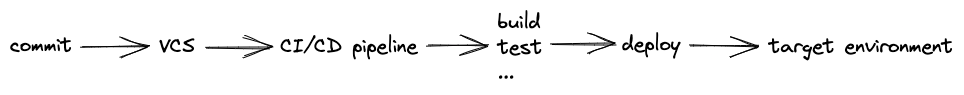
\includegraphics[width=1.00\linewidth]{assets/push-based-cd.png}
%	\caption{Push based Continuous Deployment.
	%		%		(\citeauthor{ref}, \citeyear{ref}).
	%	}
%	\label{fig:pushBasedCD}	
%\end{figure}

\begin{figure}
	\centering
	
	\noindent
	\begin{minipage}{.5\textwidth}
		\centering
		\begin{tikzpicture}[node distance=1.3cm]
			\node (start) [startstop] {Start};
			\node (one) [process, below of=start] {commit};
			\node (two) [process, below of=one] {test};
			\node (three) [process, below of=two] {build \& push artifact};
			\node (four) [process, below of=three] {deploy artifact};
			\node (stop) [startstop, below of=four] {Stop};
			
			\draw [arrow] (start) -- (one);
			\draw [arrow] (one) -- (two);
			\draw [arrow] (two) -- (three);
			\draw [arrow] (three) -- (four);
			\draw [arrow] (four) -- (stop);
		\end{tikzpicture}
		\captionof{figure}{Push-based deployment.}
		\label{tikz:push-based-cd}
	\end{minipage}%
	\begin{minipage}{.5\textwidth}
		\centering
		\begin{tikzpicture}[node distance=1.3cm]
			\node (start) [startstop] {Start};
			\node (one) [process, below of=start] {commit};
			\node (two) [process, below of=one] {test};
			\node (three) [process, below of=two] {build \& push artifact};
			\node (four) [process, below of=three, yshift=-0.8cm] {detect new desired state};
			\node (five) [process, below of=four] {GitOps engine};
			\node (six) [process, below of=five] {deploy artifact};
			\node (stop) [startstop, below of=six] {Stop};
			
			\draw [arrow] (start) -- (one);
			\draw [arrow] (one) -- (two);
			\draw [arrow] (two) -- (three);
			\draw [arrow] (five) -- (four);
			\draw [arrow] (five) -- (six);
			\draw [arrow] (six) -- (stop);
		\end{tikzpicture}
		\captionof{figure}{Pull-based deployment.}
		\label{tikz:pull-based-cd}
	\end{minipage}
	
\end{figure}

%\subsection{Pull-based Deployments}

With the GitOps approach and appropriate tools which implement its principles and pattern,
the deployment process works in a pull-based manner.
This means, that the GitOps engine, which often lives inside the deployment environment
continuously watches the desired state for changes,
and if changes occur, the new desired state is reconciled with the actual state, in order for them to match again.
Because the deployment process is not done by a task at the end of the CI/CD pipeline,
the pipeline ends with a successful push of the artifact to a registry.
At this point, typically a version updating tool like e.g. Flux Image Update Automation, which notices, that a new version is available in
the artifact registry, patches that new version into the desired state stored in the GitOps repository.
Next, the GitOps engine notices the change in the desired state and does the reconciliation,
which finally ends up in a deployment.
The processes that are responsible for deployment with the GitOps approach run asynchronously.










\section{Promotion of Releases across Environments}

When a Continuous Deployment setup consists of multiple deployment environments,
the process is usually to first deploy to the first environment,
and if the deployment succeeds, the second environment is deployed to.
Environments can also be seen as stages in this context,
where previous stages need to pass, before subsequent stages are passed through.

With the push-based deployments described in the previous section \ref{theoretical-background:gitops-cd},
where the host process of a CI/CD pipeline typically knows the state of each deployment,
it is not that big of a challenge to incorporate more deployment environments.
For critical environments, that might be required to have a human approve new releases,
the deployment task of the pipeline configuration could be set to manual.
Via the CI/CD system's interface, these deployments can be easily managed.

With the GitOps approach and pull-based deployments described in the previous section \ref{theoretical-background:gitops-cd},
the process of deploying to multiple environments is more tricky with the currently available tools.
While deploying the same new release or version of an application to multiple environments is not a problem,
the promotion of a release to other or subsequent environments, depending on if the deployment to the first environment succeeded,
is a bit of a challenge.

As previously described, the problem is that the pull-based deployment process with GitOps is asynchronous.
Once the CI/CD pipeline process uploads the artifact to the registry, the pipeline usually ends at that point.
The component responsible for deployment is the GitOps engine, which is watching the desired state,
and will pick up and continue the asynchronous deployment process, once it detects a new change in the desired state.
There is usually an automated process which updates the desired state with the new artifact's version.

\subsection{Image Update Automation}

For the popular GitOps tools like Flux or Argo,
there are components available with a functionality to update the desired state
of a particular container image version with the currently latest available, or some other specification, like a semantic version specification.

\begin{figure}[h]
	\centering
	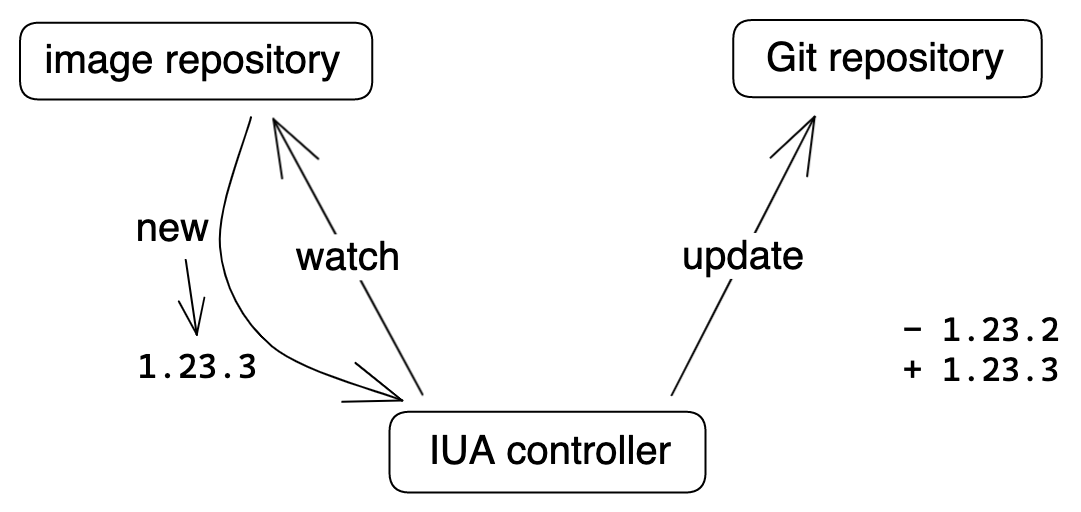
\includegraphics[width=0.72\linewidth]{assets/image-update-automation-illustration.png}
	\caption{Image Update Automation.
		%		(\citeauthor{ref}, \citeyear{ref}).
	}
	\label{fig:image-update-automation-illustration}	
\end{figure}

It works the following way: A controller continuously watches the repository/registry of the container image for new versions.
If the controller detects a new version with the specification it is configured (e.g. stable-*, 1.13.*),
it will take that new verion tag and patch it to a declared container image which is specified in one or more YAML files in a Git repository.
This tool makes it possible to achieve simple Continuous Deployment,
meaning that a commit, a code change, by a developer can automatically be released to production.
Ideally tests are run before releasing, in order to ensure quality.
When the application is deployed to multiple environments, which is specified by multiple desired state declarations,
i.e. folders in the GitOps repository, or separate repositories,
such an image update automation can be configured for all environments.
However, such a setup has its downsides.
Namely, that the new release will be deployed to all environments at once.
This is not always desired, and sometimes it is required to have some sort of manual release process between environments.

With the currently available tools in the GitOps ecosystem,
it is not straight-forward how you would setup such a promotion process,
when multiple deployment environments are required.
While it is not too difficult to achieve with push-based deployments and CI/CD,
it is currently a challenge with pull-based deployments and GitOps.

\subsection{Promotion Strategies}

An automated workflow for release promotion between environments,
can be achieved in multiple ways,
however there is no common or uniform practice for it at the moment.
Depending on the used GitOps and CI/CD systems used for a particular project or organization,
such a setup for promoting releases with multiple deployment environments can differ much.
Replacing a component in the setup, e.g. the CI/CD system or Git provider, can be quite challenging.

\begin{figure}[h]
	\centering
	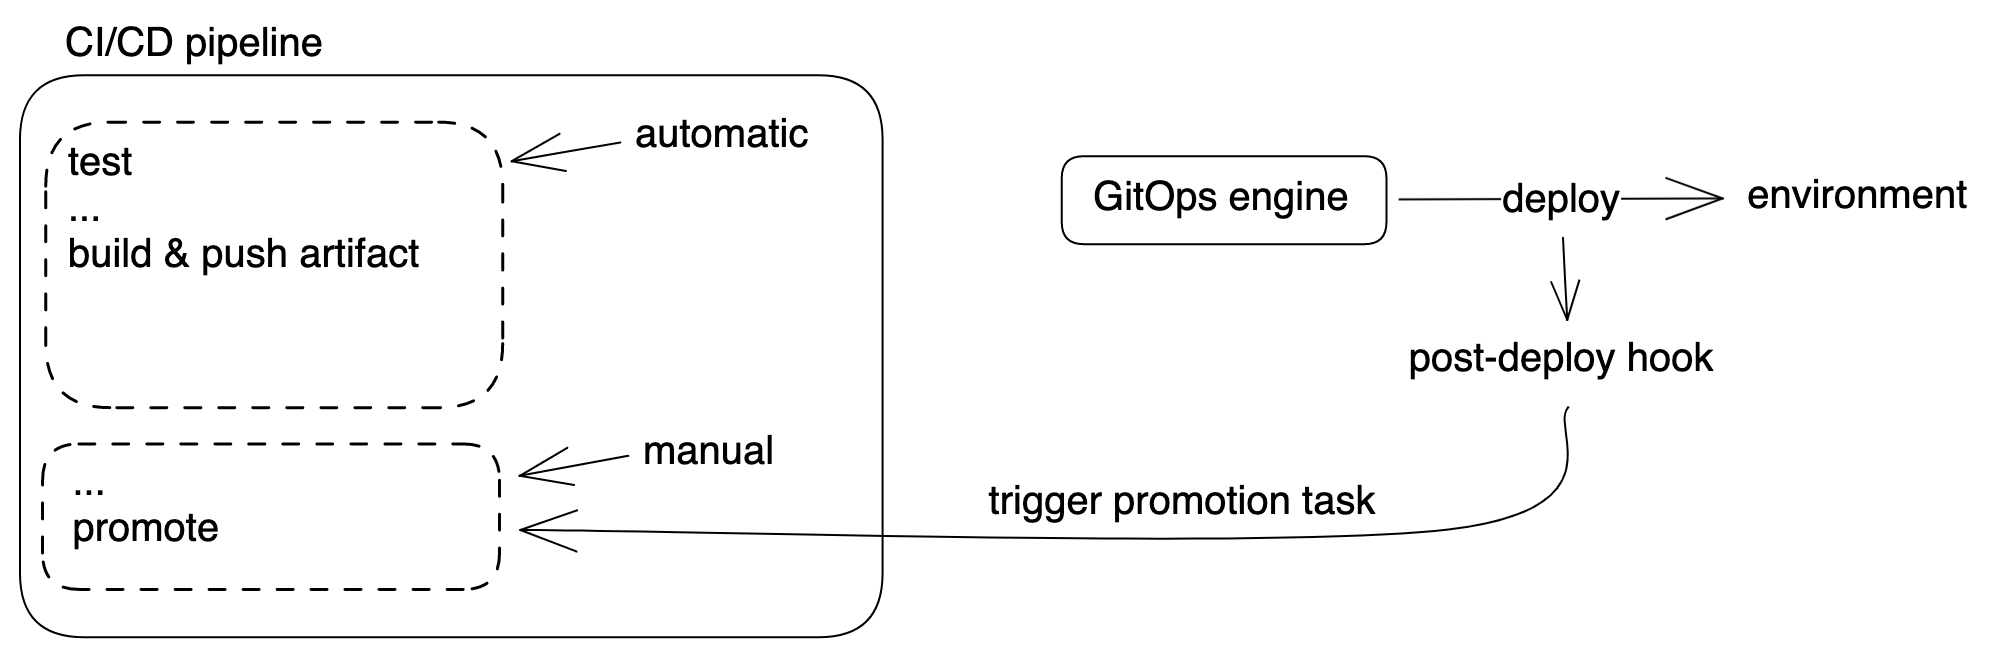
\includegraphics[width=0.99\linewidth]{assets/promotion-by-pipeline-task-post-deploy-hook.png}
	\caption{Promotion via post-deploy hook and pipeline task.
		%		(\citeauthor{ref}, \citeyear{ref}).
	}
	\label{fig:promotion-by-pipeline-task-post-deploy-hook}	
\end{figure}

A way to do a GitOps promotion is to have a pipeline task, which can be a shell script,
do some particular operation. This pipeline task could be configured to accept an incoming webhook,
upon which it would be executed.
The GitOps engine could be configured to execute a post-deployment hook,
which it would run after a successful deployment to a particular environment.
This hook could send a request to the pre-configured pipeline task, which would then be executed,
and do the GitOps promotion.












\section{Progressive Delivery \& Short-Living Environments}

With progressive delivery tools like
Flagger
\autocite{flaggerWebsite}
and
Argo Rollouts
\autocite{argoRolloutsWebsite},
which offer advanced deployment strategies
like canary and blue/green deployments, or A/B testing,
it is now easier to ensure a bad release does not impact the end users
as drastically.
As an example, the named tools make it possible to release new versions
to 10 percent of a specific region of end users,
then this canary rollout is automatically tested and evaluated against metrics,
if certain objectives for metrics fail to be met,
the new release can automatically be rolled back.

\begin{figure}[h]
	\centering
	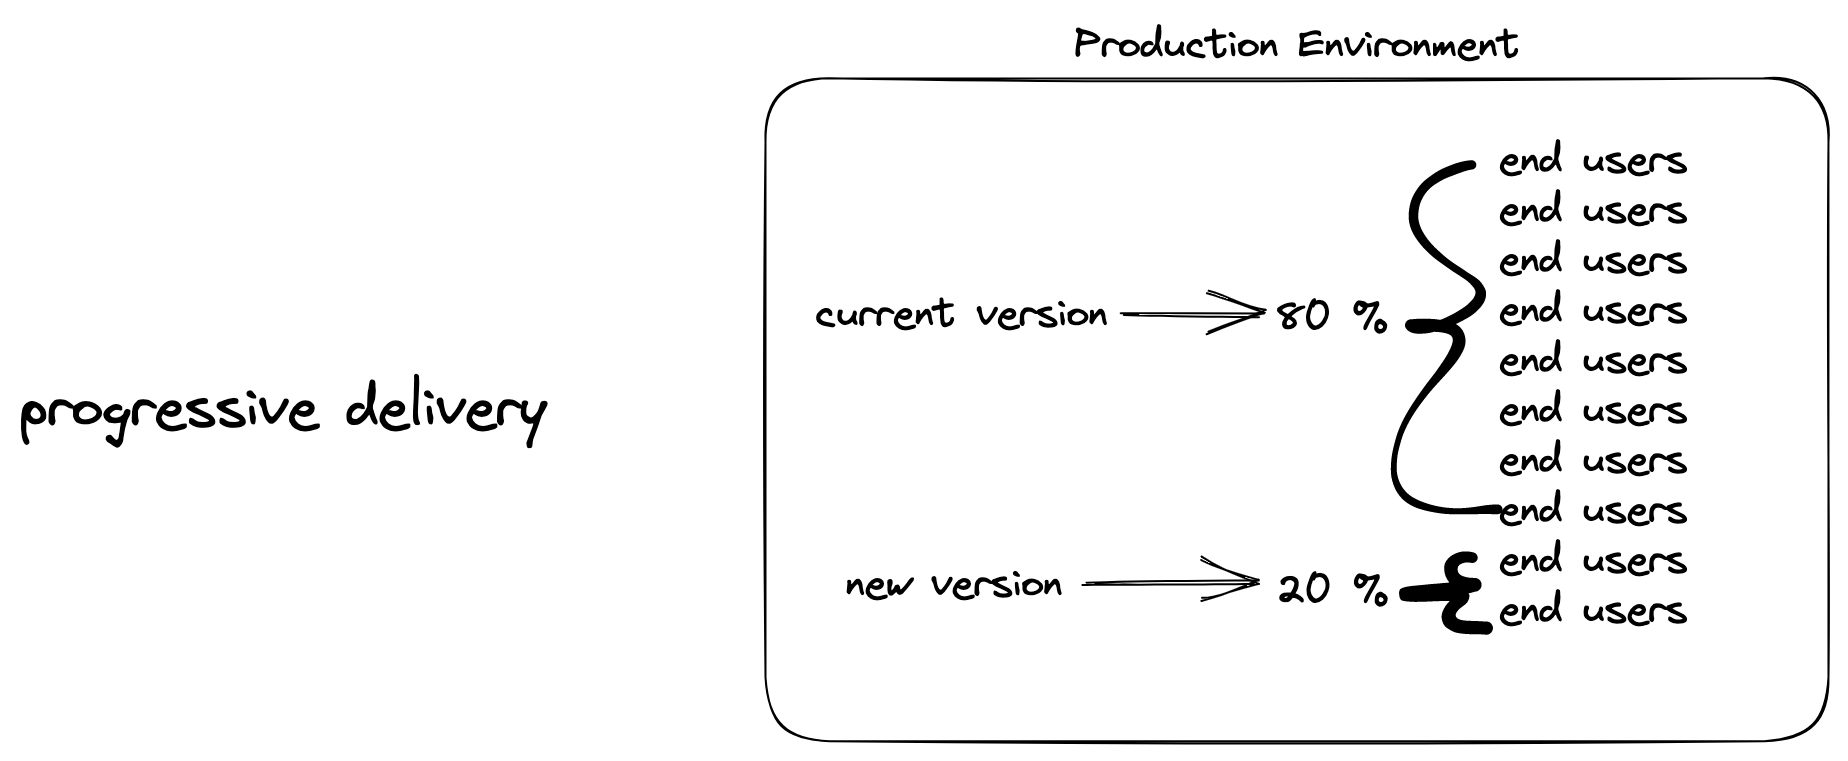
\includegraphics[width=0.75\linewidth]{assets/progressive-delivery.png}
	\caption{Example of gradual version rollout with progressive delivery.
		%		(\citeauthor{ref}, \citeyear{ref}).
	}
	\label{fig:progressive-delivery}	
\end{figure}

Since the progressive delivery tools allow for a more
fine-grained segmentation
of a single environment based on numerous parameters like
client device type, user region, user type (e.g., developer, admin),
registered or unregistered users, etc.
the requirements to have a multitude of deployment environments
have decreased for some organizations.
In combination with feature flagging functionality,
certain new features can e.g. only be released to certain users.
An illustration can be seen in fig. \ref{fig:progressive-delivery}.

The described segmentation of an environment with the progressive delivery
tools, however might not be possible for every use case or organization.
Financial institutions for example, where the requirement for absolutely zero
errors hitting the production environment is top priority and business critical,
to say the least,
may still want to run multiple environments next to progressive delivery tools,
to ensure an even higher quality and level of caution.
This is illustrated in fig. \ref{fig:deploy-multiple-envs}.

Multiple environments typically mean a big increase in costs;
with progressive delivery the need for multiple environments has decreased,
and this way costs can be reduced.

\begin{figure}[h]
	\centering
	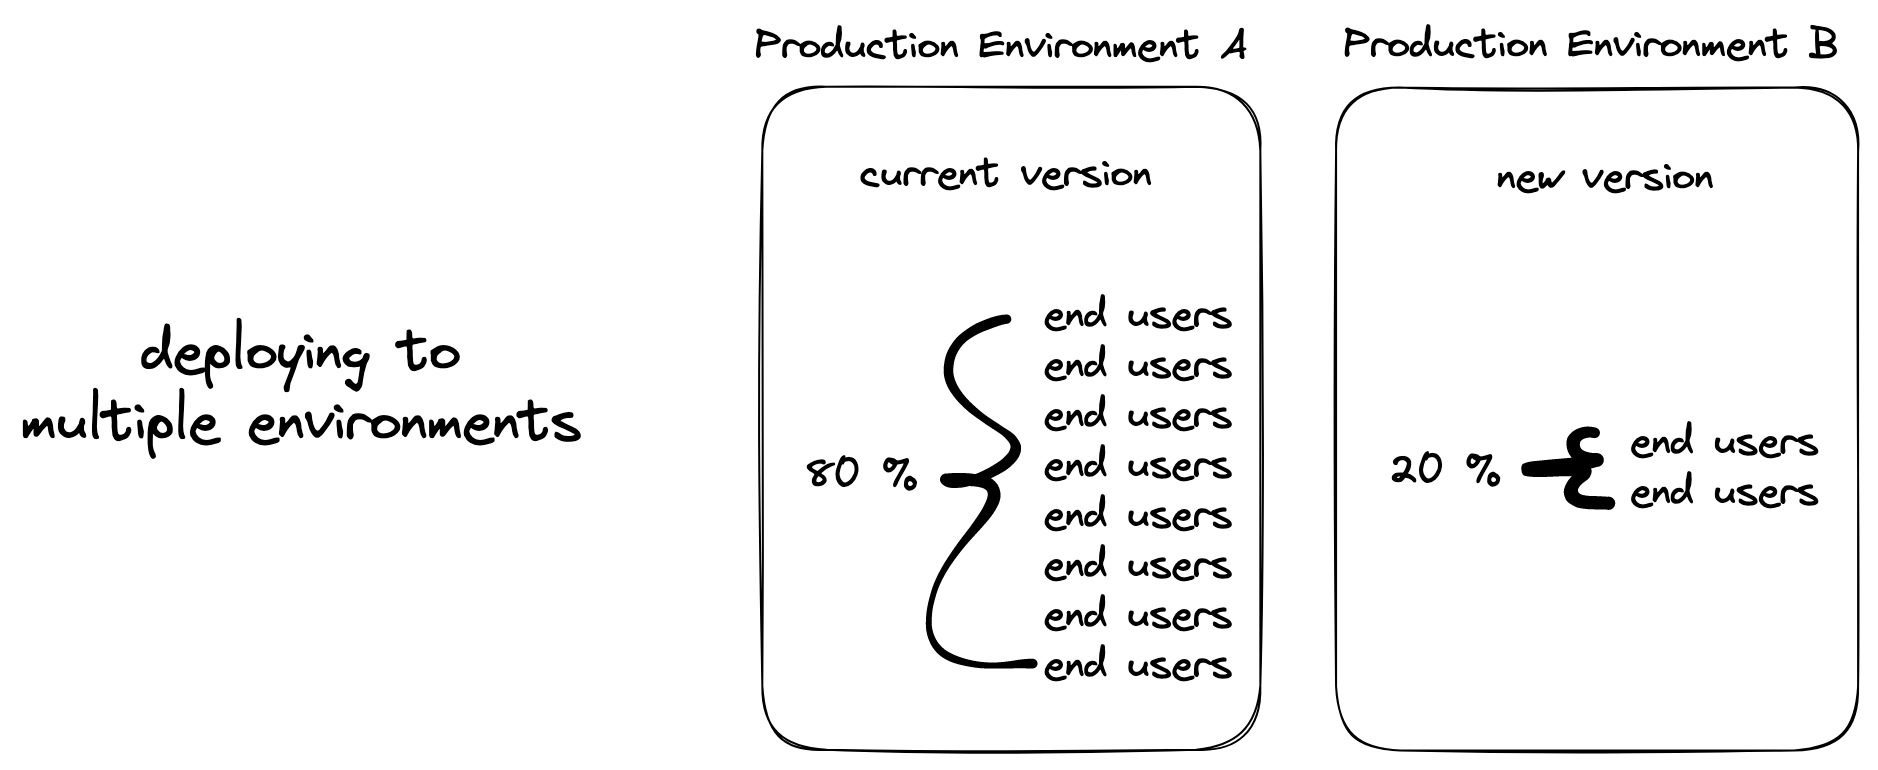
\includegraphics[width=0.75\linewidth]{assets/deploy-multiple-envs.png}
	\caption{Example of version rollout with multiple environments.
		%		(\citeauthor{ref}, \citeyear{ref}).
	}
	\label{fig:deploy-multiple-envs}	
\end{figure}

Nowadays with the rapid development and releasing of new versions,
there has become a need for dynamic, short-living environments.
% TODO: evidence for short-living environments
For every commit of an individual developer,
a deployment environment may be provisioned for previewing the changes
in a live environment that resembles the production environment as well as possible.
This short-living environment may be deleted after a short specified amount of time
has passed.






\section{Kubernetes and its extensible Architecture}
\label{theoretical-background:kubernetes}

The following section is about
the role Kubernetes plays in the current cloud native ecosystem,
and the extensible architecture of Kubernetes.

%Since the birth of the cloud native computing foundation (CNCF) in 2015 and the release of Kubernetes as the first CNCF project,
%there have emerged more than a hundred projects.
%Most of the projects are hosting cloud native technologies and tools to support Kubernetes.
%The current ecosystem and toolchains are strongly centered around Kubernetes,
%although not strictly tied to it and often times with the explicit effort
%for the ability to support alternative cloud native platforms and solutions.

\enquote*{Kubernetes, also known as K8s, is an open-source system for automating deployment, scaling, and management of containerized applications.}
\autocite{kubernetesIoWebsite}
Although this is the primary use case of Kubernetes,
and the reason why it was created initially,
Kubernetes is increasingly being used as a base cloud native platform,
to build other applications and platforms on top of.
The architecture of Kubernetes provides a solid framework and platform,
which is easily extensible.
Developers may extend its API by specifying custom resources and controllers.

There are several advantages when extending the Kubernetes API,
in comparison to a plain REST API.
Some of those are the following
\autocite{kubebuilderBookWebsite}:

\begin{itemize}
	\item \enquote*{Hosted API endpoints, storage, and validation.}
	\item \enquote*{Rich tooling and clis such as kubectl and kustomize.}
	\item \enquote*{Support for Authn and granular Authz.}
	\item \enquote*{Support for API evolution through API versioning and conversion.}
	\item \enquote*{Facilitation of adaptive / self-healing APIs that continuously respond to changes in the system state without user intervention.}
	\item \enquote*{Kubernetes as a hosting environment}
	\autocite{kubebuilderBookWebsite}
\end{itemize}

When developing a Kubernetes-native application,
many of the common capabilities which are often required for all applications,
are being provided by Kubernetes itself, or otherwise easily consumable and integrated.
These may include resource quotas, observability, monitoring, logging and tracing,
configuration state storage, declarative APIs, control loops, and event and message queueing.

\subsection{Extending Kubernetes}
% https://kubernetes.io/docs/concepts/extend-kubernetes/
Kubernetes offers several different extension points and extension patterns.
Most extension patterns however share the same basic design and principles.
In general, a custom extension is a program which reads and/or writes
to the Kubernetes API. By doing that it can provide useful automation.
Since Kubernetes is based around a declarative API,
where resources are defined as the desired state,
and controllers are responsible for continuously reconciling this
desired state with the actual state,
it has shown to be a good pattern to design custom extensions in the same way
\autocite{extendKubernetes}.

\subsection{Custom Resources, Controllers and Operators}
% https://kubernetes.io/docs/concepts/architecture/controller/
The concept of a controller and control loop within Kubernetes refers to the
meaning from robotics and automation, where
\enquote*{a control loop is a non-terminating loop that regulates the state of a system.}
\autocite{controllersKubernetes}
Controllers in Kubernetes are continuously running in a control loop,
in specified intervals and sometimes internal or external triggers, 
and watch the actual state of the cluster,
and make changes to it by interacting with the API,
in order to bring the actual state closer to the desired state,
like specified in the declarative definition.
It is typically a good practice to have one controller
be responsible for one resource, 
in order to help with separation of concerns.
Controllers make changes to resources inside the cluster,
like pods and deployments,
but can also be responsible for resources external to the cluster,
like APIs of the infrastructure provider
\autocite{controllersKubernetes}.
A typical controller implementation can be seen in figure
\ref{fig:typicalControllerKubernetes}.
As an example here, the deployment controller continuously ensures the desired state
of three replicas; if it notices the desired state and actual state differ
from one another, it does necessary actions to make them match again.
When a controller has specific domain knowledge,
or does certain tasks, which would usually be done by a human "operator",
it is called an operator.

\begin{figure}[h]
	\centering
	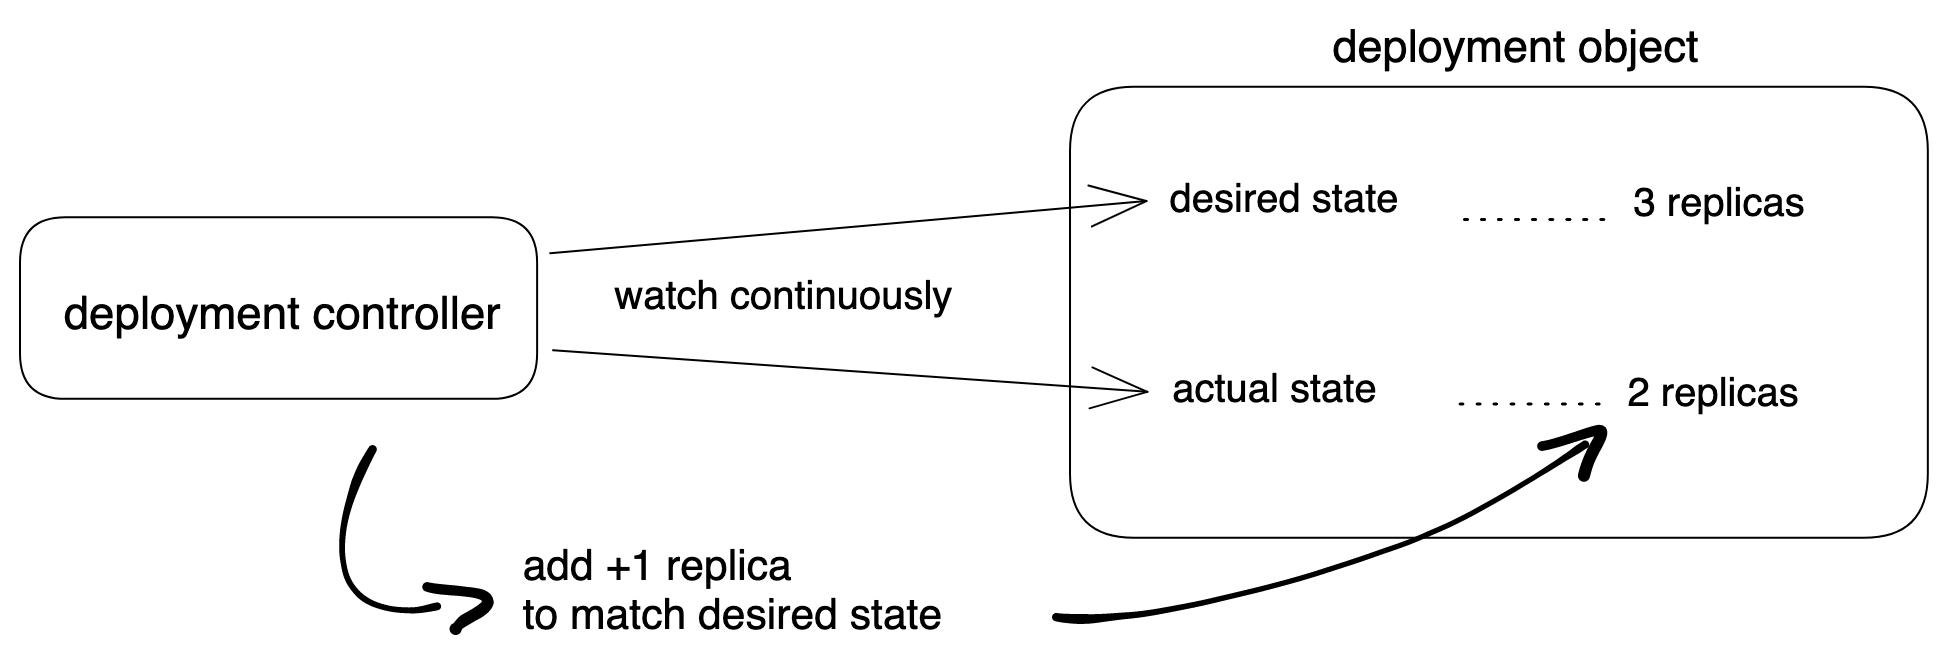
\includegraphics[width=1.00\linewidth]{assets/typical-controller.png}
	\caption{typical controller in Kubernetes.
		%		(\citeauthor{ref}, \citeyear{ref}).
	}
	\label{fig:typicalControllerKubernetes}	
\end{figure}

% https://kubernetes.io/docs/concepts/extend-kubernetes/operator/
Operators typically are a set of controllers and custom resources
with specific codified domain knowledge.
All operational tasks -
which would otherwise have to be done by a human operator -
are written in code.
This code, the controller logic, can then be automated.
Examples for such operational tasks are
backups and restoring of backups, error remediation, database migrations, etc.
\autocite{operatorWhitepaperV1}.
In overly simplified terms:
\textbf{An operator is a controller plus domain-specific operational knowledge.}
\autocite{operatorWhitepaperV1}

%\begin{figure}[h]
%	\centering
%	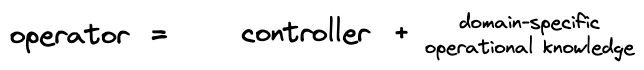
\includegraphics[width=0.85\linewidth]{assets/operator-is-controller-domain-knowledge.png}
%	\caption{Operator and Controller.
%		%		(\citeauthor{ref}, \citeyear{ref}).
%	}
%	\label{fig:operatorAndController}	
%\end{figure}

The Operator Design Pattern represents a set of principles about
managing complex applications and/or infrastructure resources,
using domain-specific knowledge.
The goal is to limit any manual work that needs to be done,
and try to automate all operational tasks.
This is done by capturing domain-specific knowledge in code,
defining the desired state of resources and exposing them
via a declarative API
\autocite{operatorWhitepaperV1}.

To simplify the process of creating and maintaining Kubernetes-native application
in the form of an operator,
there exist several operator frameworks.
The most prominent framework is the Kubebuilder Framework.
%\url{https://github.com/kubernetes-sigs/kubebuilder}
The Kubebuilder framework makes the process of extending the Kubernetes API
an easy process for developers.
An initial project can easily be boostrapped, allowing the developer to focus
on implementing the custom resource definitions and controller logic.
Any needed Kubernetes primitives, such as service accounts and RBAC permissions
are automatically generated.
Documentation for the OpenAPI resources are also generated from the code,
which is the Go programming language.
There exist rich libraries for interfacing with Kubernetes components,
since Kubernetes itself is also implemented in the Go language
\autocite{kubebuilderBookWebsite}.

With custom resources, the Kubernetes API can dynamically be extended during runtime,
without the need to access its source code or recompile it.
While a resource is
\enquote*{an endpoint in the Kubernetes API that stores a collection of API objects of a certain kind}
\autocite{customResourcesKubernetesIO},
a custom resource is
\enquote*{an extension of the Kubernetes API that is not necessarily available in a default Kubernetes installation}
\autocite{customResourcesKubernetesIO}.
Custom resources can be dynamically registered and independently updated.
Users can interface with its objects as they do with the Kubernetes built-in resources
\autocite{customResourcesKubernetesIO}.









\section{Modeling of GitOps Environments}

GitOps environments as defined in section
\ref{theoretical-background:general-definitions},
can be modeled using different approaches.
The most prominent approach is to have a folder in a Git repository
per environment. This is straight-forward and easily compatible with
the currently most used configuration and templating tools like Kustomize and Helm.
Promotion would be just a file copy operation from one to another file or folder.
However, for some promotions it is desired to only update a specific part of a file,
with a specific type of information, e.g. patching a container image tag in a Kubernetes
deployment resource.
For each environment, or only critical ones, there could be a completely separate Git repository.
Having a separate repository opens up the possibility to have a more strict separation of concerns,
regarding permissions and access rights.
Anyone who has access to a Git repository has read access to the entire repository tree.
While the write access could potentially be limited by administrators or maintainers
to certain folders, the read access will always be open for anyone who has access to the repository.

Another approach is to have a Git branch per environment.
Promotion would be a Git merge from one to another branch.
When taking this approach, and also having environment-specific configuration,
it is possible, when not being careful, that a merge conflict happens,
and the promotion would need to be solved manually.
However when this approach is purely used for the purpose of staging,
meaning environments are identical, but new releases are deployed to some environments first
after other ones,
it could in theory provide a seamless way of promotion by solely leveraging the built-in merge mechanism in Git.
Branches can usually be restricted or limited to certain developers only,
which would make it easier to implement the access permissions than the folder-per-environment approach.

This research focuses primarily on the modeling of folder-per-environment.
The designed and developed operator prototype is based on this folder-per-environment model.
However, if the requirement for branch-per-environment modeling exists in the future,
support for it can potentially be added.







%
%\section{Promotion Strategies with Existing Tools}
%
%There are many ways for achieving a promotion process when using the GitOps approach for the Continuous Delivery of
%an application or any other infrastructure declared in code.
%When a push-based CI/CD pipeline is already in place, it is often the first thing that comes to mind
%to just append the GitOps deployment as a synchronized process to the end of the pipeline.
%GitOps engines like ArgoCD offer the capability for the user to configure webhook receivers
%which reconcile an application. This makes it possible to setup a synchronous pipeline,
%which results in every code change being delivered through a pipeline step by step in a synchronous manner.
%After the push-based synchronous deployment step succeeds in the pipeline process,
%the pipeline developer can configure another imperative step which triggers reconcilication for another environment.
%
%However, there is a downside when choosing to go with such a push-based imperative approach.
%In fact, this approach would abide by the core principles of GitOps,
%namely the principle of desired state being continuously being pulled by the GitOps engine/agent.
%So the advantage of drift detection and automatic mending, would no longer be given.
%
%When following the GitOps approach, it may be desirable to decouple Continuous Integration/Delivery and Continuous Deployment.
%This means that a code change, namely a Git commit, triggers a Continuous Integration pipeline,
%which ends in a step which builds and pushes an artifact of the new version to an artifact registry.
%The pipeline ends at this point.
%Afterwards the GitOps engine, another system than the CI/CD system, is responsible for detecting the new desired state and starting reconciliation.
%However, the desired state first needs to be changed after a new artifact is available,
%and especially when multiple environments are needed and promotion should be achieved between them,
%this is not straight-forward with this asynchronous process.
%It may be desirable to trigger tests after a deployment to a certain environment is done,
%and only afterwards promote to another environment.
%The GitOps approach proposes to have the source of truth in the Git repository as the desired state of a system.
%
%Currently there is insufficient tooling in the GitOps ecosystem for streamlining such a
%multi-environment promotion process.
%
%{\color{red}\larger TODO review section!}



















\section{Summary}

In this chapter,
the theoretical background on the topic was presented.
General definitions of terms including GitOps and
releases, promotions, and environments in the context of GitOps were defined.
It was explained, how many times the term GitOps is misunderstood,
and that GitOps is actually defined in the OpenGitOps project.
The meaning of DevOps was mentioned.
GitOps related tooling and components were presented.
It was shown how GitOps changes the architecture and process of Continuous Deployment,
and how the promotion of releases is achieved without and with the GitOps approach.
Emerging patterns like progressive delivery,
as well as the concept behind short-living environments were described.
The power of Kubernetes as a cloud native platform and its use cases beyond container orchestration were presented.
Finally it was shown how the declarative representations of GitOps environments are typically modelled currently.
































%
%\section{Instruction included in the original FHBgld word processor template}
%\subsection{General definitions}
%Die in dieser Formatvorlage beispielhaft enthaltenen Überschriften sind auf die im
%konkreten Fall tatsächlich passenden Überschriften anzupassen.
%In diesem Teil der Arbeit werden die zum eindeutigen Verständnis unbedingt
%erforderlichen Grundlagen und Definitionen sowie die Erklärung wichtiger Begriffe
%angeführt.
%Die Gliederungspunkte müssen möglichst prägnant bezeichnet werden.
%\subsection{Related work / state of research}
%Auch die neuesten Entwicklungen und Arbeiten auf diesem Gebiet (Stand der
%Wissenschaft oder auch state-of-the-art) sind darzulegen, wobei diese je nach Thema
%auch in der 1. Gliederungsebene behandelt werden können.
%
%\section{Ordinary text}
%% A '%' character causes TeX to ignore all remaining text on the line,
%% and is used for comments like this one.
%
%% sections are begun with similar 
%% \subsection and \subsubsection commands.
%
%The ends  of words and sentences are marked by spaces. It doesn't matter how many 
%spaces    you type; one is as good as 100.  The
%end of   a line counts as a space.
%
%One   or more   blank lines denote the  end 
%of  a paragraph.  
%
%Since any number of consecutive spaces are treated
%like a single one, the formatting of the input
%file makes no difference to
%\LaTeX,                % The \LaTeX command generates the LaTeX logo.
%but it makes a difference to you.  When you use 
%\LaTeX \cite{lamport94},  % \cite inserts a reference, which you define at the end of the document
%making your input file as easy to read
%as possible will be a great help as you write 
%your document and when you change it.  This sample 
%file shows how you can add comments to your own input 
%file.
%
%Because printing is different from typewriting,
%there are a number of things that you have to do
%differently when preparing an input file than if
%you were just typing the document directly.
%Quotation marks like
%``this'' 
%have to be handled specially, as do quotes within
%quotes:
%``\,`this'            % \, separates the double and single quote.
%is what I just 
%wrote, not  `that'\,''.  
%
%Dashes come in three sizes: an 
%intra-word 
%dash, a medium dash for number ranges like 
%1--2, 
%and a punctuation 
%dash---like 
%this.
%
%A sentence-ending space should be larger than the
%space between words within a sentence.  You
%sometimes have to type special commands in
%conjunction with punctuation characters to get
%this right, as in the following sentence.
%Gnats, gnus, etc.\ all  % `\ ' makes an inter-word space.
%begin with G\@.         % \@ marks end-of-sentence punctuation.
%You should check the spaces after periods when
%reading your output to make sure you haven't
%forgotten any special cases.  Generating an
%ellipsis
%\ldots\               % `\ ' is needed after `\ldots' because TeX 
%% ignores spaces after command names like \ldots 
%% made from \ + letters.
%%
%% Note how a `%' character causes TeX to ignore 
%% the end of the input line, so these blank lines 
%% do not start a new paragraph.
%%
%with the right spacing around the periods requires
%a special command.
%
%\LaTeX\ interprets some common characters as
%commands, so you must type special commands to
%generate them.  These characters include the
%following:
%\$ \& \% \# \{ and \}.
%
%In printing, text is usually emphasized with an
%\emph{italic}  
%type style.  
%
%\begin{em}
%	A long segment of text can also be emphasized 
%	in this way.  Text within such a segment can be 
%	given \emph{additional} emphasis.
%\end{em}
%
%It is sometimes necessary to prevent \LaTeX\ from
%breaking a line where it might otherwise do so.
%This may be at a space, as between the ``Mr.''\ and
%``Jones'' in
%``Mr.~Jones'',        % ~ produces an unbreakable interword space.
%or within a word---especially when the word is a
%symbol like
%\mbox{\emph{itemnum}} 
%that makes little sense when hyphenated across
%lines.
%
%Footnotes\footnote{This is an example of a footnote.}
%pose no problem.
%
%\LaTeX\ is good at typesetting mathematical formulas
%like
%\( x-3y + z = 7 \) 
%or
%\( a_{1} > x^{2n} + y^{2n} > x' \)
%or  
%\( AB  = \sum_{i} a_{i} b_{i} \).
%The spaces you type in a formula are 
%ignored.  Remember that a letter like
%$x$                   % $ ... $  and  \( ... \)  are equivalent
%is a formula when it denotes a mathematical
%symbol, and it should be typed as one.
%Furthermore you can add a formula as Images or Tables, see Formula  \hyperref[eq:abc]{\ref{eq:abc}}
%\begin{equation}
%	\label{eq:abc}
%	a+b=c
%\end{equation}
%
%It is sometimes necessary to prevent \LaTeX\ from
%breaking a line where it might otherwise do so.
%This may be at a space, as between the ``Mr.''\ and
%``Jones'' in
%``Mr.~Jones'',        % ~ produces an unbreakable interword space.
%or within a word---especially when the word is a
%symbol like
%\mbox{\emph{itemnum}} 
%that makes little sense when hyphenated across
%lines.
